\documentclass[crop,tikz]{standalone}% 'crop' is the default for v1.0, before it was 'preview'
%\usetikzlibrary{...}% tikz package already loaded by 'tikz' option
\begin{document}
\usetikzlibrary{shapes,snakes}
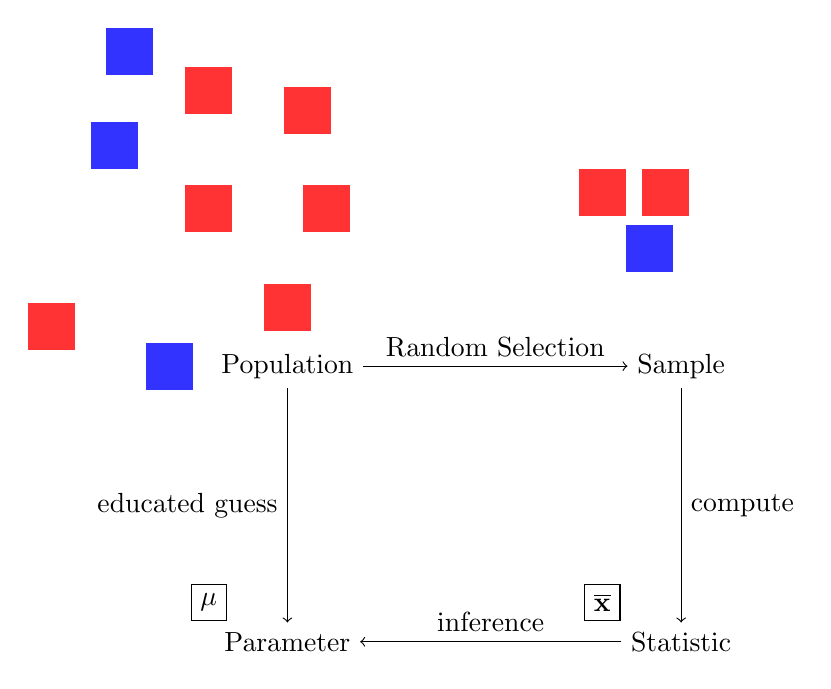
\begin{tikzpicture}

\tikzstyle{population1}=[rectangle,fill=red!80,minimum size=17pt,inner sep=0pt]
\tikzstyle{population2}=[rectangle,fill=blue!80,minimum size=17pt,inner sep=0pt]
\tikzstyle{box}=[rectangle,draw=black]


%get labels.
\node (pop) at (1,-2.) {Population};
\node[population1] (pop1) at (0., 0.) {};
\node[population1] (pop2) at (1.25, 1.25) {};
\node[population2] (pop3) at (-1., 2.) {};
\node[population1] (pop4) at (1., -1.25) {};
\node[population1] (pop5) at (0., 1.5) {};
\node[population2] (pop6) at (-0.5, -2) {};
\node[population1] (pop7) at (-2., -1.5) {};
\node[population1] (pop8) at (1.5, 0.) {};
\node[population2] (pop9) at (-1.2, .8) {};


\node (sample) at (6.,-2.) {Sample};
\node[population1] (sam1) at (5.8, 0.2) {};
\node[population1] (sam1) at (5., 0.2) {};
\node[population2] (sam1) at (5.6, -0.5) {};


\node (stat)  at ( 6,-5.5) {Statistic};
\node[box] (mean)  at ( 5, -5) {$\overline{\mathbf{x}}$};

\node (param) at ( 1, -5.5) {Parameter};
\node[box] (mean)  at ( 0, -5) {$\mu$};

\draw [->] (pop) -- (sample) node[midway, above] {Random Selection};
\draw [->] (sample) -- (stat) node[midway, right] {compute};
\draw [->] (stat) -- (param) node[midway, above] {inference};
\draw [->] (pop) -- (param) node[midway, left] {educated guess};

\end{tikzpicture}
\end{document}